\documentclass[12pt, a4paper, brazil]{abntex2}
\usepackage[utf8]{inputenc}
\usepackage[T1]{fontenc}
\usepackage[left=2cm, top=3cm, right=2cm, bottom=2cm]{geometry}
\usepackage[normalem]{ulem}
\usepackage[dvipsnames]{xcolor}
\usepackage{graphicx}
\graphicspath{{./src/img/}}
\usepackage{float}

\usepackage[alf]{abntex2cite}

\usepackage{hyperref}
\hypersetup{
    colorlinks=true,
  linkcolor=black,
  citecolor=black,
  urlcolor=black
  }

\usepackage{indentfirst}
\usepackage{multicol}

\setlength{\columnseprule}{0.5pt}
\setlength{\columnsep}{25pt}

\usepackage{amsmath}
\usepackage{amsthm}
\usepackage{amsfonts}
\usepackage{amssymb}
\usepackage{xfrac}

\usepackage{enumitem}

\DeclareMathOperator{\sen}{sen}
\DeclareMathOperator{\tg}{tg}

\renewenvironment{proof}{\vspace{\onelineskip} \noindent{\bfseries Demonstração:}}{\qed}

\setcounter{tocdepth}{2}

\newcounter{questaovest}

\newcommand{\vest}[1]{\stepcounter{questaovest}\item[\textbf{Questão \arabic{questaovest}} (#1):]}
\setlist[enumerate]{
    align=left,
    leftmargin=*,
    }
    
\setlist[enumerate,2]{
    label=\alph*),
    font=\bfseries,
    itemsep=0.1pt,
    labelsep=0em,
    parsep=0pt,
    leftmargin=1.2em
    }
    
    
    \renewcommand{\bibsection}{%
  \chapter*[Referências]{Referências} % Na página e no cabeçalho
  \addcontentsline{toc}{chapter}{Referências} % No Sumário
  }

  \chapterstyle{companion}
  \renewcommand{\printchaptertitle}[1]{
  \begin{adjustwidth}{}{0pt}
    \raggedleft\chaptitlefont#1\par\nobreak,
  \end{adjustwidth}
}



\begin{document}
  \begin{multicols*}{2}
    \begin{enumerate}
          \vest{IFBA-2018} Abaixo estão duas retas paralelas cortadas por duas transversais e um triângulo retângulo. Então, o valor da área de um quadrado de lado ''$y$'' u.c., em unidades de área, é?

            \begin{figure}[H]
                \centering
                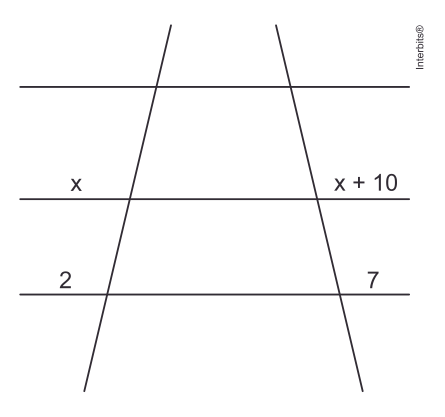
\includegraphics[width=0.4\textwidth]{q01fig01.png}
            \end{figure}

            \begin{figure}[H]
                \centering
                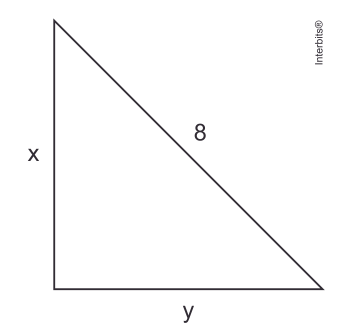
\includegraphics[width=0.4\textwidth]{q01fig02.png}
            \end{figure}

            \begin{enumerate}
                \item $48$
                \item $58$
                \item $32$
                \item $16$
                \item $28$
                %gabarito: A
            \end{enumerate}

        \columnbreak\vest{Cesgranrio-1996} Na Figura a seguir, $AB$ e $CD$ são paralelos. Se $AB=136$, $CE=75$ e $CD=50$. Quanto mede o segmento $CE$?

            \begin{figure}[H]
                \centering
                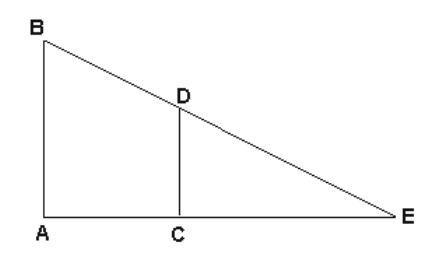
\includegraphics[width=0.4\textwidth]{q02fig1.png}
            \end{figure}

            \begin{enumerate}
                \item 136
                \item 306
                \item 204
                \item 163
                %gabarito: c
            \end{enumerate}

        \vest{ESPM-2017} Uma senhora foi ao shopping e gastou a metade do dinheiro que tinha na carteira e pagou R\$ 10,00 de estacionamento. Ao voltar para casa parou numa livraria e comprou um livro que custou a quinta parte do que lhe havia sobrado, ficando com R\$ 88,00.

        Se ela tivesse ido apenas à livraria e comprado o mesmo livro, teria restado:

            \begin{enumerate}
                \item R\$ 218,00
                \item R\$ 186,00
                \item R\$ 154,00
                \item R\$ 230,00
                \item R\$ 120,00
            \end{enumerate}

        \columnbreak\vest{ENEM-2ª apl-2010} A corrida de rua cresce no Brasil. Nunca se falou tanto no assunto como hoje, e a quantidade de adeptos aumenta progressivamente, afinal, correr traz inúmeros benefícios para a saúde física e mental, além de ser um esporte que não exige alto investimento financeiro.
        
        Um corredor estipulou um plano de treinamento diário, correndo 3 quilômetros no primeiro dia e aumentando 500 metros por dia, a partir do segundo. Contudo, seu médico cardiologista autorizou essa atividade até que o corredor atingisse, no máximo, 10 km de corrida em um mesmo dia de treino. Se o atleta cumprir a recomendação médica e praticar o treinamento estipulado corretamente em dias consecutivos, pode-se afirmar que esse planejamento de treino só poderá ser executado em, exatamente,

            \begin{enumerate}
                \item 12 dias
                \item 13 dias
                \item 14 dias
                \item 15 dias
                \item 16 dias
            \end{enumerate}

    
        \columnbreak\vest{ESPEcEx/AMAN-2013} Na figura abaixo está representado o gráfico de uma função real do 1º grau $f(x)$.

            \begin{figure}[H]
                \centering
                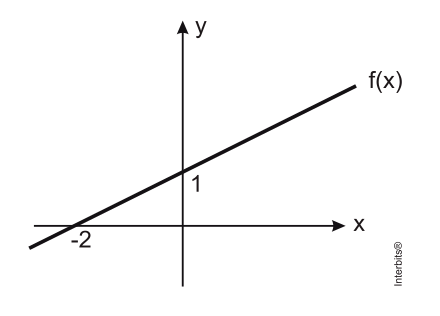
\includegraphics[width=0.4\textwidth]{q06fig.png}
            \end{figure}

        A expressão algébrica que define a função inversa de $f(x)$ é:

            \begin{enumerate}
                \item $\displaystyle y = \frac{x}{2} + 1$ \vspace{2pt}
                \item $\displaystyle y = x + \frac{1}{2}$ \vspace{6pt}
                \item $\displaystyle y = 2x - 2$ \vspace{2pt}
                \item $\displaystyle y = -2x + 2$ \vspace{2pt}
                \item $\displaystyle y = 2x+2$
            \end{enumerate}
    \end{enumerate}
  \end{multicols*}
\end{document}